% Conference-template version. Generated from ../paper.tex (same text and numbers) by ../make_cvpr.py. Do not edit by hand.
\documentclass[10pt,twocolumn,letterpaper]{article}
\usepackage[review]{cvpr}
\usepackage{graphicx}
\usepackage{booktabs}
\usepackage{adjustbox}
\usepackage{amsmath}
\usepackage{multirow}
\usepackage{rotating}
\usepackage{xcolor}
\definecolor{cvprblue}{rgb}{0.21,0.49,0.74}
\usepackage[pagebackref,breaklinks,colorlinks,allcolors=cvprblue]{hyperref}
\setlength{\tabcolsep}{4pt}
\def\paperID{*****} % TODO: replace with the OpenReview paper ID
\def\confName{CVPR}
\def\confYear{2027}

\title{How Much Is a Real Fall Worth? Staged, Synthetic, Labelled and Unlabelled Real Video for Fall Detection}
\author{Anonymous submission}

\begin{document}
\maketitle
\begin{abstract}
Video fall detectors are usually trained and evaluated on falls staged by actors, where they score near perfectly. We ask which training data prepares a detector for real falls, and whether real video has to be labelled to be useful. We build \textbf{FallOrNot}, a test set sampled from OOPS!\ accident videos independently of any model and labelled for whether a person falls, so that \emph{other accidents} act as false-alarm negatives; we also test on OmniFall's in-the-wild split (OF-ItW) and on HMDB51. With frozen CLIP and VideoMAE features, staged-trained probes that score 1.00 in-domain reach 0.76 AUROC on FallOrNot, synthetic training 0.81 and 131 hand-labelled real falls 0.90, but on HMDB51 the ranking flips and synthetic training is best. Our main result is that much of the benefit of real data needs no labels. Accident videos come with the time at which something goes wrong, so the clip before it is a free real non-fall. Starting from the synthetic-trained probe, we pseudo-label 7,063 unlabelled accident clips, add the free negatives, and retrain on real clips only. Under a success rule fixed before any result, this zero-label probe beats synthetic training on FallOrNot ($0.894$ vs.\ $0.814$) and OF-ItW ($0.937$ vs.\ $0.872$), equals a probe trained on 125 hand-labelled falls, and is the best probe on HMDB51 ($0.953$). Controls locate the gain: a random-start version still reaches $0.865\pm0.011$ on FallOrNot, so most of the in-domain gain is accident-versus-ordinary-activity structure; pseudo-labelling adds fall-specific information beyond a plain accident detector, and on falls versus other accidents it beats synthetic training both in domain (all 345 hand-labelled accident clips, with their videos removed from the pool: $+0.058$, $p=0.013$; rule fixed in advance) and out of domain ($p=0.005$). The same zero-label training set also trains an end-to-end fine-tuned VideoMAE: $0.910\pm0.004$ on FallOrNot over three seeds, above synthetic fine-tuning ($0.838$, significant for every seed) and level with fine-tuning on our hand labels ($0.902$). A variant that also labels each accident by what follows it (is a person on the ground?) did not improve the method. With a few labels, a probe anchored to the synthetic solution is never meaningfully worse than the better single source. Tests fixed in advance that were not met are reported.
\end{abstract}

%=====================================================================
\section{Introduction}
Falls are the second-leading cause of unintentional injury death worldwide, and about 71\% of fall deaths occur in people aged 60 or older~\cite{who_falls}; long periods on the floor after a fall are associated with worse outcomes~\cite{fleming2008}. Camera-based fall detection promises automatic alerts without wearables, and published detectors often report near-perfect accuracy. Most of that evidence comes from staged datasets in which young actors fall onto mattresses in front of fixed cameras~\cite{kwolek2014,charfi2013}.

Real falls are different: they are sudden, partly occluded, filmed from arbitrary viewpoints, and embedded among other abrupt events such as collisions, dropped objects and people catching themselves. OmniFall~\cite{omnifall} recently showed a large drop from staged to in-the-wild falls on fall-containing OOPS!~\cite{epstein2020oops} videos, and argued that synthetic training videos generalise better than staged ones. This leaves practical questions open for anyone building a detector: \emph{how much real data is needed, is real data worth more than synthetic data, does the answer change with the test set, how often do detectors raise alarms for accidents that are not falls, and does real video have to be labelled at all?}

The last question matters most in practice, because labelling is the bottleneck: we hand-labelled 165 test videos and 268 training clips, while OOPS!\ contains thousands of accident videos that nobody has labelled for falls. Those videos are not unstructured, however. Each comes with the time at which something goes wrong, so the seconds before it show ordinary activity, a \emph{real non-fall that costs nothing}. We show that this timing signal, combined with pseudo-labels from a detector that has never seen a real fall, trains a probe without any human label that matches hand-labelled training on our test set and transfers better to an independent source than either hand-labelled real or synthetic training. We then take the result apart with controls fixed in advance, and report where it holds and where it does not.

\paragraph{Contributions.}
\begin{enumerate}\setlength\itemsep{1pt}
\item \textbf{Zero-label adaptation} (\cref{sec:nolabel}). From 7,063 unlabelled accident clips and their free pre-accident negatives, a probe trained with no human label reaches 0.894, 0.937 and 0.953 AUROC on three test sets (synthetic-only: 0.814, 0.872, 0.917), under a success rule committed before any result. It is worth about 125 hand-labelled falls in domain, and fine-tuning VideoMAE on the same zero-label data matches fine-tuning on our hand labels (0.910 vs.\ 0.902 on FallOrNot; rule fixed in advance, met).
\item \textbf{Controls that locate the gain.} A random-start control and a plain accident detector show that most of the in-domain gain is accident-versus-ordinary-activity structure, that pseudo-labelling adds fall-specific information beyond it, and that it separates falls from \emph{other accidents} better than synthetic training without any label, in domain ($p=0.013$, rule fixed in advance) and out of domain ($p=0.005$).
\item \textbf{FallOrNot}, a real-world test set sampled from \emph{all} annotated OOPS!\ accidents independently of any model, so that non-fall accidents are hard false-alarm negatives; its labels agree with OmniFall's on 27 of 28 shared videos.
\item A controlled comparison of \textbf{staged, synthetic and hand-labelled real training data} on three test sets, showing that the ranking of labelled sources \textbf{flips between real-world test sets}, for frozen probes and fine-tuned models.
\item For the few-label case, an \textbf{anchored probe} that is never meaningfully worse than the better single source from 4 to 125 real falls (rule fixed in advance, met on two test sets), and an ablation showing that for fine-tuning the same benefit comes simply from starting at the synthetic-trained model (\cref{sec:anchor}).
\item A record of all eight tests specified in advance, including the three that were not met (one of them a new consequence-based labelling method), plus a compilation leakage check and a second-annotator study.
\end{enumerate}

%=====================================================================
\section{Related work}
\paragraph{Staged and simulated falls.} UR Fall~\cite{kwolek2014}, Le2i~\cite{charfi2013} and the Multiple Cameras Fall Dataset~\cite{auvinet_mcfd} are widely used staged sets on which detectors approach ceiling performance. For wearable accelerometers, algorithms tuned on simulated falls lose accuracy on real-world falls~\cite{bagala2012,klenk2016}; we study the analogous question for video.

\paragraph{Learning with weak or no labels.} Weakly supervised fall detection trains from video-level labels with multiple-instance learning~\cite{wu2023weakfall,madsen2024weakfall}; a human still labels every video. Multiple-instance learning from video-level labels is also the standard formulation of weakly supervised video anomaly detection~\cite{sultani2018anomaly}. Self-training with pseudo-labels~\cite{xie2020noisystudent} is a standard way to use unlabelled data, and unsupervised domain adaptation has been applied to fall detection across sensing modalities, from labelled RGB to unlabelled depth video with thresholded pseudo-labels~\cite{xiao2023umafd}; the OOPS!\ paper itself studies self-supervised representations learned from unlabelled video~\cite{epstein2020oops}. Pseudo-labels from CLIP's zero-shot predictions have been used to adapt image classifiers without labels~\cite{huang2022upl}, and accident anticipation in dashcam video takes its supervision from the annotated time of the accident~\cite{chan2016dashcam}. Our zero-label experiment (\cref{sec:nolabel}) uses self-training in a setting we have not seen studied for falls: the unlabelled data are web accident videos, and the only supervision taken from them is the accident time that OOPS!\ already provides, which yields real non-falls at no labelling cost. We do not propose a new learning algorithm; the contribution is the supervision source, the measurement of what it is worth in hand labels, and controls that separate the timing signal from the pseudo-labels.

\paragraph{In-the-wild video.} OOPS!~\cite{epstein2020oops} contains about 20k web videos of unintentional actions with annotated transition times. \textbf{OmniFall}~\cite{omnifall}, the closest work, unifies eight staged datasets, adds 12k synthetic videos (OF-Syn) and an in-the-wild test set of 818 fall-containing OOPS!\ videos (OF-ItW), shows a large staged-to-wild drop, finds synthetic training better than staged, and reports an upper-bound model trained with in-the-wild data. We do not claim to be first to show the staged-to-wild gap. Our work differs in (i) asking whether real accident video can be used \emph{without} labels, (ii) negatives drawn from all accidents by a model-independent sample, (iii) the question of how much labelled real data is needed and whether it beats synthetic data at equal budget, and (iv) testing every conclusion on an independent real-world source.

\paragraph{Encoders.} We use CLIP~\cite{radford2021clip} through OpenCLIP~\cite{openclip} with DataComp weights~\cite{gadre2023datacomp}, and VideoMAE~\cite{tong2022videomae} fine-tuned on Kinetics-400~\cite{kay2017kinetics}.

%=====================================================================
\section{The FallOrNot test set}
\paragraph{Source and clips.} We use the 10,961 OOPS!\ videos whose transition time $t$ was found by at least two annotators (median used). Each video yields an \emph{event} clip $[t-1, t+1]$\,s and, when $t\ge3.5$\,s, a \emph{pre-event} clip $[t-3.5, t-1.5]$\,s of ordinary activity. Every clip, in every dataset in this paper, is 2\,s long and sampled at 16 frames.

\paragraph{Model-independent test sample.} A video enters the test sample if the MD5 hash of its name falls below a fixed threshold (about 600 videos; 422 with usable clips). Selection depends on no model, so the benchmark cannot favour any detector. Clips were labelled in a fixed random order, so any labelled prefix is itself a random sample.

\paragraph{Labels.} Following the WHO definition, a fall is an event in which a person inadvertently comes to rest on the ground, floor or another lower level~\cite{who_falls}. The annotator answered \emph{fall}, \emph{not a fall} (including other accidents, near-falls and animals) or \emph{unsure} (excluded). Positives are event clips labelled \emph{fall}; negatives are event clips labelled \emph{not a fall} (hard negatives) and the pre-event clips of labelled test videos (easy negatives).

\paragraph{Size.} 165 test videos are labelled (255 clips, 102 falls). A separate training pool, the 3,000 event clips with the highest zero-shot CLIP fall score (never overlapping the test sample), provides 268 labelled real training clips from 180 videos (131 falls). The pool is model-selected and used only for training.

\paragraph{Second annotator.} An independent second annotator labelled 100 of the test videos without seeing the first annotator's answers. On the 98 clips both labelled \emph{fall} or \emph{not a fall}, raw agreement was 0.796 and Cohen's $\kappa=0.498$ [0.297, 0.678] (moderate). Disagreements were asymmetric: in 16 of 20 cases the second annotator saw a fall where the first did not (\cref{sec:annotator}).

%=====================================================================
\section{Experimental setup}\label{sec:setup}
\paragraph{Training data.} \emph{Staged}: UR Fall~\cite{kwolek2014}; fall clips are centred on the frames labelled ``falling'', negatives are pre-fall clips and 2\,s windows (1\,s stride) over the activity videos; 316 clips, 60 falls (30 falls $\times$ 2 cameras). \emph{Synthetic}: OmniFall OF-Syn~\cite{omnifall}; one clip per video, centred on the fall segment for all 2,136 videos containing a fall and on the longest segment for 3,000 hash-sampled videos without one. \emph{Real}: the 268 labelled OOPS!\ training clips.

\paragraph{External real-world test: HMDB51.} HMDB51~\cite{kuehne2011hmdb} is independent of OOPS!. From its split~1 (100 clips per class) we use all 100 human-labelled \texttt{fall\_floor} clips and 20 hash-sampled clips from each of the other 50 classes. A hard subset, fixed in advance, keeps falls and whole-body or ground-contact actions (cartwheel, flic-flac, somersault, handstand, dive, jump, sit, sit-up, push-up, stand, climb; 320 clips). Clips are covered by 2\,s windows every 1\,s and scored by their maximum window. Nothing is trained on HMDB51.

\paragraph{Representations and detectors.} \emph{CLIP appearance}: mean of 8 L2-normalised CLIP ViT-L/14 frame embeddings. \emph{CLIP temporal}: [mean, last-third minus first-third, mean absolute frame-to-frame change]. \emph{VideoMAE}: pooled VideoMAE-B (Kinetics-400) embedding of 16 frames. \emph{CLIP + VideoMAE}: concatenation of the last two. Detectors are zero-shot CLIP (fall vs.\ non-fall prompt margin, prompts fixed in advance) and L2-regularised logistic regression on standardised features ($C=0.1$, class-balanced).

\paragraph{Fine-tuning.} VideoMAE-B fine-tuned end to end with hyper-parameters fixed before any run: 5 epochs, batch 8, AdamW, learning rate $5\times10^{-5}$, weight decay 0.05, one-cycle schedule, class-balanced sampling, horizontal flips, last checkpoint; trained on synthetic (1,000 + 1,000 clips), real (268 clips) or both; three seeds.

\paragraph{Metrics and statistics.} AUROC, average precision and recall at 5\% false-positive rate, with 95\% confidence intervals from a bootstrap (1,000 resamples). OOPS!\ videos are cut from YouTube compilations, and clips from one compilation are correlated, so on FallOrNot we resample whole compilations (see the leakage check in \cref{sec:leak}); on HMDB51 we resample clips. Two detectors are compared on the same clips with a paired bootstrap of the same kind (2,000 resamples), which gives the difference, its 95\% CI and a two-sided $p$-value. $p$-values are not adjusted for multiple comparisons; apart from the eight tests specified in advance (fine-tuning, source-balanced mixing, the anchored probe, anchored fine-tuning, zero-label adaptation, the extended hard test, zero-label fine-tuning and consequence-guided labelling), all comparisons are exploratory.

\paragraph{Tests specified in advance.} For each of these eight tests we committed the success rule, with all settings, to the project repository before the corresponding run; the rules are stated where the results are reported. For fine-tuning the rule was that training on synthetic + real data must beat the best frozen probe on \emph{both} FallOrNot and HMDB51, with the paired 95\% CI above zero. Nothing was registered with an external registry.

%=====================================================================
\section{Which labelled training data?}
\subsection{Staged training does not transfer}
All staged-trained probes reach AUROC $\ge0.998$ in five-fold cross-validation on UR Fall (grouped by sequence), and zero-shot CLIP reaches 0.912. On FallOrNot the same probes reach 0.723--0.765 (\cref{tab:fallornot}), and the best catches 30\% of falls at 5\% false positives (VideoMAE, recall 0.304). In-domain staged numbers cannot rank methods: every probe is at ceiling.

\begin{table}[t]\centering\small
\caption{AUROC on \textbf{FallOrNot} (255 clips, 102 falls) by training data. Zero-shot CLIP: 0.717. Best per row in bold. Runs 3--4, 10.}
\label{tab:fallornot}
\begin{adjustbox}{max width=\linewidth}
\begin{tabular}{lcccc}\toprule
Representation & Staged & Synthetic & Real & Syn.\ + real\\\midrule
CLIP appearance & 0.723 & 0.728 & 0.732 & \textbf{0.800}\\
CLIP temporal & 0.728 & 0.795 & \textbf{0.866} & 0.823\\
VideoMAE & 0.765 & 0.789 & 0.787 & \textbf{0.842}\\
CLIP + VideoMAE & 0.759 & 0.814 & \textbf{0.899} & 0.872\\\midrule
\multicolumn{5}{l}{\footnotesize CLIP + VideoMAE 95\% CIs: staged [0.698, 0.814]; synthetic [0.753, 0.869];}\\[-2pt]
\multicolumn{5}{l}{\footnotesize real [0.858, 0.935]; synthetic + real [0.825, 0.914].}\\\bottomrule
\end{tabular}
\end{adjustbox}
\end{table}

\subsection{On FallOrNot, a few real falls beat thousands of synthetic ones}
With CLIP + VideoMAE, real training beats staged training by $+0.139$ [$+0.085$, $+0.193$] ($p<0.001$) and synthetic training by $+0.085$ [$+0.030$, $+0.137$] ($p=0.001$). Synthetic training scores higher than staged, the direction OmniFall reports~\cite{omnifall}, but the difference is not significant here ($+0.054$ [$-0.000$, $+0.110$], $p=0.053$; CLIP temporal $+0.067$, $p=0.030$). Adding synthetic data to real data does not help this representation ($-0.027$, $p=0.19$).

\emph{Motion is what benefits from real data.} Real training helps CLIP temporal ($+0.138$ [$+0.073$, $+0.198$] over staged, $p<0.001$) but not CLIP appearance ($+0.009$, $p=0.76$) or VideoMAE alone ($+0.022$, $p=0.49$).

\emph{Equal budget} (\cref{fig:budget}): training on $k$ falls plus $k$ non-falls from one source, synthetic data plateaus near 0.82 from about 125 falls up to all 2,136 (0.812--0.825), staged data stays near 0.75, and real data keeps rising: 30 real falls (0.836 $\pm$ 0.018) already exceed every synthetic budget, and about 8 real falls match the whole staged set. With only 4 falls, real data is unreliable (0.670 $\pm$ 0.130).

\begin{figure}[t]\centering
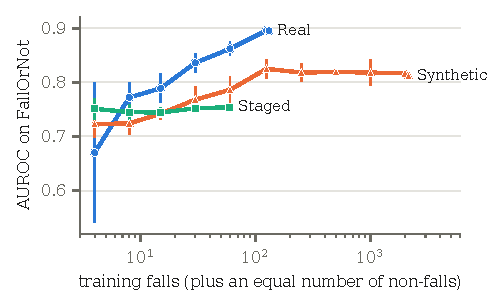
\includegraphics[width=\columnwidth]{fig_budget.pdf}
\caption{Equal training budget, CLIP + VideoMAE probes, FallOrNot test set (mean $\pm$ s.d.\ over random draws). Run 4.}
\label{fig:budget}
\end{figure}

\paragraph{Falls vs.\ other accidents.} Restricted to accident-moment clips (165 clips, 102 falls), CLIP + VideoMAE reaches 0.715 (staged), 0.772 (synthetic), 0.860 (real) and 0.848 (synthetic + real); zero-shot CLIP reaches 0.686. Telling a fall from another accident remains the hardest part of the task.

\paragraph{Compilation leakage check.}\label{sec:leak} Of the 268 real training clips, 111 come from a compilation that also contributes test clips. Retraining on the 157 clips (77 falls) from compilations absent from the test set gives 0.866, against $0.874\pm0.014$ for random subsets of the same size and class counts We find no clear evidence that shared compilations inflate the real-data result.

\subsection{A third, larger test set with independent labels}\label{sec:ofitw}
To check the FallOrNot result at larger scale and with labels that are not ours, we score the same probes on OmniFall's in-the-wild test split (OF-ItW~\cite{omnifall}): 571 OOPS!\ videos annotated by OmniFall's team, from which we cut 1,671 clips (636 falls; one clip per fall segment, and one per other segment of at least 1\,s that is not ``fallen'' and does not overlap a fall). Our 20 real training clips from these videos are removed. \Cref{tab:ofitw} confirms the FallOrNot ordering, with every step significant ($p<0.001$, paired, by compilation): synthetic over staged $+0.058$ [$+0.040$, $+0.077$], our real clips over synthetic $+0.055$ [$+0.039$, $+0.071$]. Probes trained on our 248 hand-labelled clips (0.927) come close to probes trained on OF-ItW's own 734 training clips (0.951), and on the 28 videos labelled by both teams the labels agree on 27 ($\kappa=0.78$; a small sample skewed towards falls). Simply pooling synthetic and real clips is significantly worse than real alone here ($-0.022$ [$-0.031$, $-0.013$]). OF-ItW negatives are other moments of fall videos rather than other accidents, and the footage is again OOPS!, so this is a second in-domain test, not an out-of-domain one.

\begin{table}[t]\centering\small
\caption{AUROC on the \textbf{OF-ItW test split} (1,671 clips, 636 falls; labels by OmniFall's team). ``Real (ours)'': our 248 training clips; ``Real (OF)'': OF-ItW train + val, 734 clips. Zero-shot CLIP: 0.731. Run 11.}
\label{tab:ofitw}
\setlength\tabcolsep{3.5pt}
\begin{adjustbox}{max width=\linewidth}
\begin{tabular}{lccccc}\toprule
Representation & Staged & Syn. & \shortstack{Real\\(ours)} & \shortstack{Real\\(OF)} & \shortstack{Syn.\ +\\real (OF)}\\\midrule
CLIP appearance & 0.746 & 0.727 & 0.781 & \textbf{0.829} & 0.825\\
CLIP temporal & 0.785 & 0.846 & 0.900 & \textbf{0.925} & 0.883\\
VideoMAE & 0.771 & 0.817 & 0.844 & \textbf{0.909} & 0.899\\
CLIP + VideoMAE & 0.815 & 0.872 & 0.927 & \textbf{0.951} & 0.929\\\bottomrule
\end{tabular}
\end{adjustbox}
\end{table}

\subsection{On an independent source, the ranking flips}
On HMDB51 (\cref{tab:hmdb}, \cref{fig:flip}) the real-data advantage disappears. With CLIP + VideoMAE, real training is slightly \emph{worse} than synthetic ($-0.029$ [$-0.057$, $-0.003$], $p=0.029$) and no better than staged ($-0.011$, $p=0.57$). Synthetic training rescues VideoMAE ($+0.214$ over staged, $p<0.001$), and CLIP appearance trained on real OOPS!\ data falls to 0.626. HMDB51 falls look closer to staged falls than OOPS!\ accidents do: staged probes reach 0.899 there but 0.759 on FallOrNot, and zero-shot CLIP 0.834 vs.\ 0.717. Many HMDB51 falls come from films.

\begin{table}[t]\centering\small
\caption{AUROC on \textbf{HMDB51} (1,100 clips, 100 falls; nothing trained on it). Zero-shot CLIP: 0.834. Run 5.}
\label{tab:hmdb}
\begin{adjustbox}{max width=\linewidth}
\begin{tabular}{lcccc}\toprule
Representation & Staged & Synthetic & Real & Syn.\ + real\\\midrule
CLIP appearance & 0.783 & \textbf{0.813} & 0.626 & 0.803\\
CLIP temporal & \textbf{0.887} & 0.866 & 0.825 & 0.842\\
VideoMAE & 0.664 & 0.877 & 0.779 & \textbf{0.901}\\
CLIP + VideoMAE & 0.899 & \textbf{0.917} & 0.888 & 0.901\\\midrule
\multicolumn{5}{l}{\footnotesize Hard subset (320 clips), CLIP + VideoMAE: staged 0.833, synthetic 0.880,}\\[-2pt]
\multicolumn{5}{l}{\footnotesize real 0.777, synthetic + real 0.855.}\\\bottomrule
\end{tabular}
\end{adjustbox}
\end{table}

\begin{figure}[t]\centering
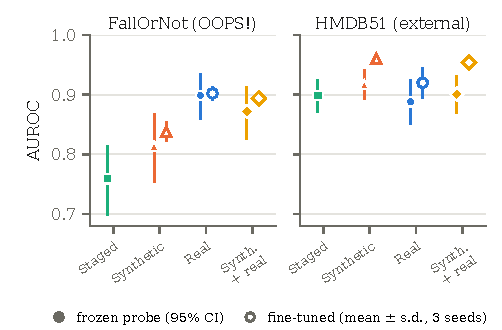
\includegraphics[width=\columnwidth]{fig_flip.pdf}
\caption{The ranking of training sources flips between real-world test sets. Filled: CLIP + VideoMAE probes with 95\% CIs (runs 4--5). Hollow: fine-tuned VideoMAE, mean $\pm$ s.d.\ over 3 seeds (run 7).}
\label{fig:flip}
\end{figure}

\subsection{Fine-tuning (test specified in advance)}
The test specified in advance was \textbf{not met} for any of three seeds. On FallOrNot, fine-tuning on synthetic + real differs from the best probe by $-0.011$ to $-0.002$; on HMDB51 by $+0.028$ to $+0.049$ (CI above zero for two of three seeds). Averaged over seeds (\cref{tab:nolabelft}, first two rows), the flip reappears: real-trained models are best on FallOrNot and synthetic-trained models are best on HMDB51; synthetic + real (0.894, 0.954, 0.890 on FallOrNot, HMDB51 and its hard subset) is within 0.008 of the best mean on both test sets.

\subsection{Which labelled source is safest?}
No single labelled source is best everywhere. Measured by the shortfall from the best source on each test (FallOrNot, its hard subset, HMDB51, its hard subset), real-only training loses up to 0.103 (probes) and 0.127 (fine-tuned) on the HMDB51 hard subset, and synthetic-only training up to 0.088 and 0.101 on FallOrNot's accident negatives, whereas synthetic + real never loses more than 0.027 (probes) or 0.032 (fine-tuned). By plain worst-case AUROC, real-only training is as good as the mixture.

\paragraph{Source-balanced mixing.} A probe in which every source-and-class cell has equal total weight had to beat the plain mixture on both test sets (rule fixed in advance). It was \textbf{not met}: balancing helps on FallOrNot ($+0.016$ [$+0.005$, $+0.028$], $p=0.004$) but not on HMDB51 ($+0.002$ [$-0.004$, $+0.008$]).

\subsection{Robustness to the annotator}\label{sec:annotator}
Re-grading FallOrNot with the second annotator's labels (99 videos, 152 clips) lowers absolute AUROC (best probe 0.797 instead of 0.899) but preserves the staged-to-real gap, real over staged training ($+0.083$, $p=0.024$), the learning-curve shape and the synthetic plateau. The in-domain advantage of real over synthetic training shrinks to $+0.065$ [$-0.006$, $+0.137$] and is no longer significant ($p=0.079$).

%=====================================================================
\section{Do the real clips need labels? Zero-label adaptation}\label{sec:nolabel}
Labelling is the expensive part of real data, so we ask how far \emph{unlabelled} real video goes. OOPS!\ annotates the time at which each video turns into an accident. That gives structure for free: the clip before the accident shows ordinary activity and is a real non-fall, while the clip at the accident is a fall or some other accident. We take every embedded OOPS!\ video that is in neither FallOrNot's test sample nor OF-ItW (7,063 accident clips, 3,473 of them with a pre-accident clip) and never read a label for them; the pool includes the videos behind our 268 labelled training clips, treated as unlabelled. The synthetic-trained probe scores the accident clips; the top 20\% become pseudo-falls, the bottom 20\% and all pre-accident clips become pseudo-non-falls, and a fresh probe is trained on these real clips alone and re-scores the pool. We repeat this three times. The fraction, the number of rounds and the probe were fixed in advance.

\paragraph{Rule fixed in advance.} Success required the zero-label probe to beat the synthetic-only probe on both FallOrNot and the OF-ItW test split with a paired 95\% interval above zero (resampled by compilation). \textbf{The rule was met} (\cref{tab:nolabel}): $+0.081$ [$+0.033$, $+0.129$] on FallOrNot and $+0.065$ [$+0.052$, $+0.077$] on OF-ItW (both $p<0.001$). On FallOrNot the zero-label probe is indistinguishable from the probe trained on our 268 hand-labelled clips ($-0.004$ [$-0.039$, $+0.031$], $p=0.83$); on OF-ItW it is slightly below the probe trained on OF-ItW's own labels ($-0.014$ [$-0.024$, $-0.003$], $p=0.009$). It closes 95\% and 82\% of the gap between synthetic and human-labelled real training, and on both test sets it matches a real-only probe trained on 125 labelled falls and 125 labelled non-falls, the largest budget on our learning curve.

\paragraph{Out of domain.} On HMDB51, which was not part of the rule, the zero-label probe scores 0.953, above synthetic-only ($+0.036$ [$+0.016$, $+0.056$], $p=0.001$) and above the human-labelled real probe (0.888). It is the only training recipe in this paper that is best or within 0.015 of the best probe on all three test sets; the ranking flip of \cref{fig:flip} does not apply to it.

\paragraph{What makes it work.} Without the pre-accident clips the gain nearly disappears (0.837 on FallOrNot, 0.875 on OF-ItW), whereas using them as the \emph{only} negatives is as good as the full method (0.896, 0.939): the free negatives are the key ingredient and the bottom-20\% accident clips are unnecessary. Adding the free negatives to synthetic data without pseudo-falls hurts (0.782, 0.843), so real pseudo-falls and real negatives are needed together. Three rounds improve on one by 0.017 and 0.013. When the pool is restricted to compilations absent from both test sets (1,110 accident clips, 16\% of the pool) the gain is smaller but remains significant ($+0.065$, $p=0.015$; $+0.054$, $p<0.001$); the smaller pool and the removal of shared compilations are confounded. Because the same web clip can appear in several compilations, we also removed every pool video whose CLIP appearance is close to any test clip (cosine above 0.95; 354 videos, threshold fixed in advance): the gain is unchanged (0.892 and 0.936; $+0.078$ and $+0.064$ over synthetic training, both $p<0.001$), and removing up to 951 videos changes in-domain AUROC by at most 0.006.

\paragraph{Control and sensitivity (exploratory).} We declared the following analysis exploratory before running it. \emph{Random start:} replacing the synthetic probe's initial scores by random numbers still gives $0.865\pm0.011$ on FallOrNot, $0.931\pm0.001$ on OF-ItW and $0.914\pm0.013$ on HMDB51 (five seeds; \cref{tab:nolabel}). Most of the in-domain gain therefore does not come from fall-specific pseudo-labels but from the structure ``accident moment versus ordinary activity'': 62\% of the accidents in FallOrNot's random sample of OOPS!\ are falls, so recognising the accident moment is already a good fall detector on these test sets. \emph{No synthetic data:} starting from CLIP's zero-shot text prompts gives 0.899, 0.936 and 0.941. \emph{Settings:} 2--5 rounds and 10--30\% pseudo-labelled stay within 0.01 of the fixed setting in domain; among pseudo-falls that happen to carry one of our labels, the share of real falls rises from 0.80 after one round to 0.96 after three ($n\approx46$). \emph{Pool size:} about 350 unlabelled videos already give 0.864 and 0.912, and gains level off beyond roughly 1,800 videos (\cref{fig:nolabel}, left).

\paragraph{Falls versus other accidents.} Does the zero-label probe only detect accidents, or does it tell falls from other accidents? We wrote down how to read this analysis before running it. On FallOrNot's hard subset (accident-moment clips only: 102 falls, 63 other accidents; \cref{fig:nolabel}, right) the zero-label probe scores 0.835, against 0.772 for synthetic training, $0.767\pm0.021$ for the random start, 0.724 for a plain accident detector (all accident clips against all pre-accident clips, no pseudo-labels) and 0.860 for the human-labelled probe. Its advantage over the accident detector is significant ($+0.112$ [$+0.044$, $+0.186$], $p=0.001$), so pseudo-labelling adds fall-specific information beyond accident timing; the random start, by contrast, learns accident detection only. Its advantage over synthetic training on this subset alone, however, is not significant ($+0.064$ [$-0.005$, $+0.131$], $p=0.065$). We therefore ran a larger test whose rule we fixed in advance: every hand-labelled accident clip (FallOrNot's 165 plus the 180 accident clips of our labelled training pool; 233 falls, 112 other accidents) is used as test data, and all of those videos are removed from the unlabelled pool before retraining. \textbf{The rule was met}: the zero-label probe reaches 0.804 against 0.746 for synthetic training ($+0.058$ [$+0.015$, $+0.103$], $p=0.013$), $0.732\pm0.019$ for the random start ($+0.049$, $p=0.005$) and 0.707 for the accident detector ($+0.098$, $p<0.001$). On FallOrNot's random sample alone the gain is now just significant ($+0.069$, $p=0.046$); on the model-selected training-pool clips alone it is not ($+0.047$, $p=0.15$). The deficit to human labels on FallOrNot's hard subset is not significant ($-0.020$ [$-0.068$, $+0.028$], $p=0.42$). On HMDB51's hard subset (falls against fall-like classes) the zero-label probe (0.920) is significantly above synthetic training ($+0.039$ [$+0.014$, $+0.066$], $p=0.005$), the random start ($+0.031$, $p=0.010$), the accident detector ($+0.036$, $p=0.031$) and the human-labelled probe ($+0.143$ [$+0.101$, $+0.185$]).

\paragraph{Fine-tuned models.} Does the zero-label data also train a video model end to end? We repeat the fixed pipeline, take the 1,000 highest-scoring accident clips as pseudo-falls and 1,000 pre-accident clips as non-falls, and fine-tune VideoMAE-B with exactly the recipe of \cref{sec:setup}, three seeds. The rule, fixed in advance, required a higher mean AUROC than synthetic fine-tuning on FallOrNot and a paired 95\% CI above zero for at least two of three seeds. \textbf{It was met} (\cref{tab:nolabelft}): $0.910\pm0.004$ against $0.838\pm0.014$, with the interval above zero for all three seeds ($+0.047$ to $+0.086$). The zero-label model is level with fine-tuning on our 268 hand-labelled clips ($0.902$; no seed differs significantly), also on FallOrNot's hard subset ($0.852$ vs.\ $0.863$). On HMDB51 it keeps the synthetic model's level ($0.959$ vs.\ $0.960$) and is above hand-labelled fine-tuning for two of three seeds ($+0.061$, $+0.050$, both $p<0.001$); on HMDB51's hard subset it is somewhat below synthetic fine-tuning ($0.893$ vs.\ $0.922$; significant for one seed).

\begin{table}[t]\centering\small
\caption{Fine-tuned VideoMAE-B, AUROC, mean $\pm$ s.d.\ (population) over three seeds. Zero-label: 1,000 pseudo-falls and 1,000 free pre-accident non-falls, no human label. Runs 6, 7 and 19.}
\label{tab:nolabelft}
\begin{adjustbox}{max width=\linewidth}
\begin{tabular}{lcccc}\toprule
Fine-tuned on & FallOrNot & FoN hard & HMDB51 & HMDB hard\\\midrule
Synthetic & $.838\pm.014$ & $.762\pm.020$ & $\mathbf{.960}\pm.005$ & $\mathbf{.922}\pm.012$\\
Real, human labels & $.902\pm.010$ & $\mathbf{.863}\pm.015$ & $.920\pm.021$ & $.795\pm.055$\\
\textbf{Zero-label} & $\mathbf{.910}\pm.004$ & $.852\pm.006$ & $.959\pm.003$ & $.893\pm.017$\\\bottomrule
\end{tabular}
\end{adjustbox}
\end{table}

\paragraph{A negative result: labelling an accident by its consequence.} After a fall the person is usually on the ground; after many other accidents they are not. We embedded the clip $[t+1, t+3]$\,s after every accident, scored it with CLIP for ``person on the ground'' against ``person upright'', and added that score to the ranking in every self-training round (prompts, window and rule fixed in advance; the detector is still tested on the 2\,s event clip only). On its own the consequence score separates falls from other accidents only weakly (AUROC 0.681 on the labelled accident clips). The rule required a significant gain over plain zero-label training on all 345 labelled accident clips; \textbf{it was not met} ($0.812$ vs.\ $0.804$, $+0.008$ [$-0.020$, $+0.036$], $p=0.60$), and out of domain the consequence signal hurt (HMDB51 0.921 vs.\ 0.952; hard subset 0.846 vs.\ 0.915). We keep the simpler method.

\begin{figure*}[t]\centering
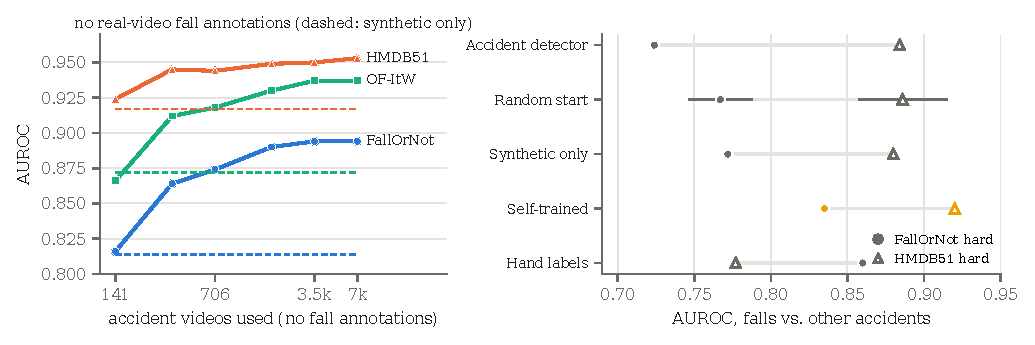
\includegraphics[width=0.92\linewidth]{fig_nolabel.pdf}
\caption{Zero-label adaptation. \emph{Left:} AUROC against the number of unlabelled accident videos used (mean of three random subsets; the full pool is the fixed setting); dashed lines are synthetic-only training. \emph{Right:} falls versus other accidents on the two hard subsets; random start is mean $\pm$ s.d.\ over five seeds. Runs 15--17.}
\label{fig:nolabel}
\end{figure*}

\begin{table*}[t]\centering\small
\caption{Zero-label adaptation (CLIP + VideoMAE probes), AUROC. No human label is read for any row except the last. ``Hard'': falls vs.\ other accidents (FallOrNot) or vs.\ fall-like classes (HMDB51). Random start: mean $\pm$ s.d.\ over five seeds. Last row: our 268 labelled clips, except OF-ItW, where it is OF-ItW's own training split. Runs 15 and 17; ``--'': not computed. The accident detector is one probe trained on all accident clips against all pre-accident clips.}
\label{tab:nolabel}
\begin{tabular}{lccccc}\toprule
Training & FallOrNot & OF-ItW & HMDB51 & FallOrNot hard & HMDB51 hard\\\midrule
Synthetic only & 0.814 & 0.872 & 0.917 & 0.772 & 0.880\\
\textbf{Zero-label (fixed setting)} & \textbf{0.894} & \textbf{0.937} & \textbf{0.953} & 0.835 & \textbf{0.920}\\
\quad 1 round instead of 3 & 0.877 & 0.924 & 0.945 & -- & --\\
\quad no pre-accident clips & 0.837 & 0.875 & 0.934 & -- & --\\
\quad only pre-accident clips as negatives & 0.896 & 0.939 & 0.951 & -- & --\\
\quad synthetic + free negatives, no pseudo-falls & 0.782 & 0.843 & 0.902 & -- & --\\
\quad pool without test-set compilations & 0.879 & 0.927 & 0.938 & -- & --\\
\quad start: CLIP zero-shot prompts, no synthetic data & 0.899 & 0.936 & 0.941 & 0.840 & 0.885\\
\quad start: random scores (control) & $0.865\pm0.011$ & $0.931\pm0.001$ & $0.914\pm0.013$ & $0.767\pm0.021$ & $0.886\pm0.029$\\
Accident detector (no pseudo-labels) & 0.849 & 0.926 & 0.882 & 0.724 & 0.884\\\midrule
Real, human labels (full pool) & 0.899 & 0.951 & 0.888 & 0.860 & 0.777\\\bottomrule
\end{tabular}
\end{table*}

%=====================================================================
\section{With a few labels: anchoring to the synthetic solution}\label{sec:anchor}
When a handful of labelled real falls exists, how should it be combined with synthetic data? A real-only probe is unstable below about 30 falls, and pooling lets thousands of synthetic clips outweigh the real ones (\cref{sec:ofitw}). We test a known form of biased regularisation~\cite{yang2007asvm,kuzborskij2013,li2018l2sp}: a probe trained on $k$ real falls and $k$ real non-falls whose weights are penalised for leaving the synthetic-trained probe's weights, with the strength chosen by cross-validation on the training clips. Under a rule fixed in advance, its mean AUROC over ten draws had to stay within 0.005 of the better of the real-only and synthetic-only probes at every $k\in\{4,8,15,30,60,125\}$ and exceed both on average, on FallOrNot and OF-ItW. \textbf{The rule was met}: averaged over budgets, 0.848 against 0.804 (real-only) and 0.814 (synthetic-only) on FallOrNot, and 0.901 against 0.867 and 0.873 on OF-ItW; with four real falls, $0.813\pm0.005$ against $0.687\pm0.124$ for real-only. The gain is confined to small budgets; with the full real pool the anchored probe is level with real-only training on FallOrNot and slightly below it on OF-ItW ($-0.008$, $p=0.002$). For end-to-end fine-tuning, starting from the synthetic-fine-tuned VideoMAE also met a rule fixed in advance (with 8 real falls, 0.826 against 0.652 for real-only fine-tuning), but an ablation showed that the penalty adds nothing there: the benefit comes from the synthetic starting point, i.e.\ plain sequential fine-tuning. Full tables are in the supplementary material.

%=====================================================================
\section{Discussion}
\paragraph{Collect real video first; label the hard cases.} Much of the value of real data lay in the video rather than in the labels: unlabelled accident clips with free pre-accident negatives recovered 82--95\% of the benefit of hand labels in domain and generalised better out of domain than hand-labelled real or synthetic data. The controls qualify this. Most of the in-domain gain is the easy part, accident versus ordinary activity, which the accident time gives away; pseudo-labelling adds fall-specific information on top, significantly but modestly in domain ($+0.058$ on falls versus other accidents) and clearly out of domain. Hand labels are therefore best spent where the free signal is silent: on accidents that are not falls. A plausible reason for the out-of-domain advantage is scale and variety (7,063 unlabelled videos against 268 labelled clips), but we did not test this.

\paragraph{Benchmarks need accident negatives.} A random-start control that never sees a fall-specific signal scores 0.931 on OF-ItW and $0.865$ on FallOrNot, but only 0.767 on FallOrNot's hard subset. A test set whose negatives are ordinary activity, or other moments of fall videos, can thus be largely solved by detecting ``something went wrong''; only non-fall accidents as negatives reveal whether a model has learned what a fall is.

\paragraph{If labels are available.} A few dozen hand-labelled real falls are worth more than thousands of synthetic falls in their own domain, but not on another source; training on both had the smallest worst-case shortfall (at most 0.03 AUROC). With only a handful of labels, anchor to the synthetic solution rather than pool.

\paragraph{One real-world benchmark is not enough.} The ranking of training sources reversed between FallOrNot and HMDB51, and the two benchmarks disagree even about how hard real falls are (staged probes: 0.759 vs.\ 0.899). Claims such as ``synthetic beats staged'' or ``real beats synthetic'' should be tested on more than one in-the-wild source.

%=====================================================================
\section{Limitations}
\begin{itemize}\setlength\itemsep{1pt}
\item \textbf{Label uncertainty.} Agreement between annotators was moderate ($\kappa=0.50$); absolute scores depend on the annotator.
\item \textbf{Scale.} FallOrNot has 165 labelled test videos (63 non-fall accidents), so its intervals are wide; OF-ItW is larger but shares the OOPS!\ source.
\item \textbf{Sources.} Real training data, the unlabelled pool and two of three test sets are OOPS!\ footage; HMDB51 falls are partly from films; no source focuses on older adults at home; UR Fall is the only staged set.
\item \textbf{Zero-label adaptation.} A random-start control recovers most of the in-domain gain; the in-domain gain on falls versus other accidents is modest ($+0.058$, $p=0.013$, on 345 clips that mix a random and a model-selected sample) and not significant on the model-selected part alone. One deterministic run with one setting fixed in advance (three seeds for fine-tuning); half of the videos have no pre-accident clip; pseudo-labelling is a known technique, and the method needs accident timestamps, which arbitrary video lacks.
\item \textbf{Anchoring} is a known form of biased regularisation; it gave no gain with the full real pool, and for fine-tuning the penalty did not matter (one test set, three draws, one penalty strength).
\item \textbf{Model-selected training pool.} The labelled real training clips were pre-selected by a CLIP zero-shot score; the test sample and the unlabelled pool were not.
\item \textbf{Many unadjusted comparisons.} Eight tests were specified in advance (five were met); the remaining $p$-values are exploratory. Fine-tuning hyper-parameters were fixed, not tuned.
\end{itemize}

\section{Conclusion}
Staged-trained fall detectors that look perfect in the lab fail on real accidents, and hand-labelled real falls fix that only in their own domain. Unlabelled accident video, pseudo-labelled from a synthetic-trained probe and combined with the free non-falls that precede every accident, gave a probe that needed no human label, matched hand-labelled training in domain to within 0.014 AUROC and was the best probe out of domain, under a success rule fixed in advance. Controls show that most of the in-domain gain comes from accident timing, that pseudo-labelling adds fall-specific information beyond it, and that it also separates falls from other accidents better than synthetic training, modestly in domain and clearly out of domain. Fine-tuning a video model on the same zero-label data matched fine-tuning on our hand labels. Fall benchmarks need non-fall accidents as negatives and more than one real-world source. We release FallOrNot's labels, timestamps and code.

\paragraph{Data and ethics.} OOPS!\ videos are public web videos; we release only labels, timestamps and code. UR Fall is licensed CC BY-NC-SA 4.0 for non-commercial research; HMDB51 is CC BY 4.0; OmniFall annotations are released for non-commercial use.

%=====================================================================
\small

\section*{LLM Usage Statement}
A large language model assistant (Claude, Anthropic) was used extensively in this work. It wrote the data-processing, feature-extraction, fine-tuning and evaluation code; proposed the experimental design, including the model-independent test sample, the additional test sets, the zero-label adaptation experiment with its controls, the tests specified in advance and the leakage check; produced the figures; searched for and summarised related work; and drafted the text of this paper. A second assistant (ChatGPT, OpenAI) was used to check bibliographic details. The human authors chose the research topic, ran every experiment, labelled the data (no label was produced by a model), recruited the second annotator, decided which experiments to run, and reviewed the results and the manuscript. All numbers in the paper are copied from logged experiment outputs, and all references were checked against their sources. The authors take full responsibility for the content of the paper.

\begin{thebibliography}{99}

\bibitem{auvinet_mcfd} E.~Auvinet, C.~Rougier, J.~Meunier, A.~St-Arnaud, and J.~Rousseau. Multiple cameras fall data set. Technical Report 1350, DIRO, Universit\'e de Montr\'eal, 2010.

\bibitem{bagala2012} F.~Bagal\`a et~al. Evaluation of accelerometer-based fall detection algorithms on real-world falls. \emph{PLoS ONE}, 7(5):e37062, 2012.

\bibitem{chan2016dashcam} F.-H.~Chan, Y.-T.~Chen, Y.~Xiang, and M.~Sun. Anticipating accidents in dashcam videos. In \emph{ACCV}, LNCS 10114, 2016.

\bibitem{charfi2013} I.~Charfi, J.~Miteran, J.~Dubois, M.~Atri, and R.~Tourki. Optimized spatio-temporal descriptors for real-time fall detection: comparison of support vector machine and Adaboost-based classification. \emph{Journal of Electronic Imaging}, 22(4):041106, 2013.

\bibitem{epstein2020oops} D.~Epstein, B.~Chen, and C.~Vondrick. Oops! Predicting unintentional action in video. In \emph{CVPR}, 2020.

\bibitem{fleming2008} J.~Fleming and C.~Brayne. Inability to get up after falling, subsequent time on floor, and summoning help: prospective cohort study in people over 90. \emph{BMJ}, 337:a2227, 2008.

\bibitem{gadre2023datacomp} S.~Y. Gadre et~al. DataComp: In search of the next generation of multimodal datasets. In \emph{NeurIPS Datasets and Benchmarks Track}, 2023.

\bibitem{huang2022upl} T.~Huang, J.~Chu, and F.~Wei. Unsupervised prompt learning for vision-language models. arXiv:2204.03649, 2022.

\bibitem{kay2017kinetics} W.~Kay et~al. The Kinetics human action video dataset. arXiv:1705.06950, 2017.

\bibitem{klenk2016} J.~Klenk et~al. The FARSEEING real-world fall repository: a large-scale collaborative database to collect and share sensor signals from real-world falls. \emph{European Review of Aging and Physical Activity}, 13:8, 2016.

\bibitem{kuehne2011hmdb} H.~Kuehne, H.~Jhuang, E.~Garrote, T.~Poggio, and T.~Serre. HMDB: A large video database for human motion recognition. In \emph{ICCV}, pages 2556--2563, 2011.

\bibitem{kuzborskij2013} I.~Kuzborskij and F.~Orabona. Stability and hypothesis transfer learning. In \emph{ICML}, PMLR 28(3):942--950, 2013.

\bibitem{kwolek2014} B.~Kwolek and M.~Kepski. Human fall detection on embedded platform using depth maps and wireless accelerometer. \emph{Computer Methods and Programs in Biomedicine}, 117(3):489--501, 2014.

\bibitem{li2018l2sp} X.~Li, Y.~Grandvalet, and F.~Davoine. Explicit inductive bias for transfer learning with convolutional networks. In \emph{ICML}, PMLR 80:2825--2834, 2018.

\bibitem{madsen2024weakfall} K.~Madsen, Z.~Li, F.~Lauze, and K.~Nasrollahi. Person fall detection using weakly supervised methods. In \emph{WACV Workshops}, pages 143--151, 2024.

\bibitem{omnifall} D.~Schneider, Z.~Marinov, M.~Mistol, Z.~Zhong, A.~Jaus, R.~D\"uger, R.~Baur, M.~S. Sarfraz, and R.~Stiefelhagen. OmniFall: From staged through synthetic to wild, a unified multi-domain dataset for robust fall detection. In \emph{ECCV}, 2026. arXiv:2505.19889.

\bibitem{openclip} G.~Ilharco, M.~Wortsman, R.~Wightman, C.~Gordon, N.~Carlini, R.~Taori, A.~Dave, V.~Shankar, H.~Namkoong, J.~Miller, H.~Hajishirzi, A.~Farhadi, and L.~Schmidt. OpenCLIP. Zenodo, 2021. doi:10.5281/zenodo.5143773.

\bibitem{radford2021clip} A.~Radford et~al. Learning transferable visual models from natural language supervision. In \emph{ICML}, 2021.

\bibitem{sultani2018anomaly} W.~Sultani, C.~Chen, and M.~Shah. Real-world anomaly detection in surveillance videos. In \emph{CVPR}, pages 6479--6488, 2018.

\bibitem{tong2022videomae} Z.~Tong, Y.~Song, J.~Wang, and L.~Wang. VideoMAE: Masked autoencoders are data-efficient learners for self-supervised video pre-training. In \emph{NeurIPS}, 2022.

\bibitem{wu2023weakfall} L.~Wu, C.~Huang, S.~Zhao, J.~Li, J.~Zhao, Z.~Cui, Z.~Yu, Y.~Xu, and M.~Zhang. Robust fall detection in video surveillance based on weakly supervised learning. \emph{Neural Networks}, 163:286--297, 2023.

\bibitem{xiao2023umafd} H.~Xiao, K.~Peng, X.~Huang, A.~Roitberg, H.~Li, Z.~Wang, and R.~Stiefelhagen. Toward privacy-supporting fall detection via deep unsupervised RGB2Depth adaptation. \emph{IEEE Sensors Journal}, 23(23):29143--29155, 2023.

\bibitem{xie2020noisystudent} Q.~Xie, M.-T.~Luong, E.~Hovy, and Q.~V. Le. Self-training with Noisy Student improves ImageNet classification. In \emph{CVPR}, pages 10684--10695, 2020.

\bibitem{yang2007asvm} J.~Yang, R.~Yan, and A.~G. Hauptmann. Cross-domain video concept detection using adaptive SVMs. In \emph{ACM Multimedia}, 2007. doi:10.1145/1291233.1291276.

\bibitem{who_falls} World Health Organization. Falls (fact sheet), 21 October 2026. \url{https://www.who.int/news-room/fact-sheets/detail/falls}, accessed November 2026.

\end{thebibliography}
\end{document}
